\documentclass{article}
\usepackage{amsmath}
\usepackage{mathtools}
\usepackage{gensymb}
\usepackage[a4paper,inner=1.5cm,outer=1.5cm,top=2cm,bottom=0.5cm]{geometry} 
\usepackage{xcolor}                    
\usepackage{tikz}                           
\usepackage{multicol}
\usepackage{pgfplots}
\usetikzlibrary{calc}
\usetikzlibrary{intersections}
\usetikzlibrary{intersections,calc,angles,quotes}
\usetikzlibrary{shapes,arrows,positioning,decorations.pathreplacing,calc}
\usetikzlibrary{calc,angles,positioning,intersections,quotes,decorations.markings}
\usepackage{tkz-euclide}
\usetikzlibrary{backgrounds}
\usetikzlibrary{calc,through}
\usetikzlibrary{angles}
\usetikzlibrary{fadings}
\usetikzlibrary{shapes.geometric}
\usetikzlibrary{shapes.symbols}
\usepackage{draftwatermark}
\usepackage{mathptmx}

\SetWatermarkText{\textcolor{black!10}{Mathema Shukur}}
\SetWatermarkFontSize{2 cm}
\usepackage[utf8]{inputenc}
\usepackage{fontspec}

\setmainfont{[Kalpurush.ttf]}
\newfontface{\en}{[Arial.ttf]} %%this is optional, if you want to use a secondary font. Any english font is supported
\newlength\Radius
\setlength\Radius{4cm}
\begin{document} 
	\Large
	\textcolor{red}{Welcome To} 
	\\
	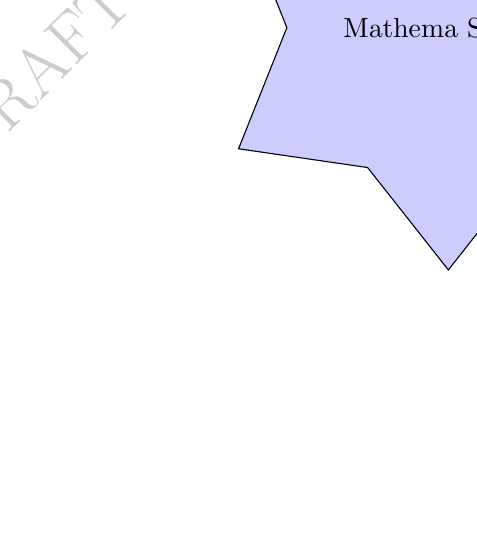
\begin{tikzpicture}
		\tikz \node [fill=blue!20,star,star points=6,draw] {Mathema Shukur };
	\end{tikzpicture}
	\\
	যাদের জন্যে প্রযোজ্যঃ  	\textcolor{magenta}{একাদশ ও দ্বাদশ শ্রেণীর শিক্ষার্থী} \\
	বিষয়ঃ \textcolor{magenta}{উচ্চতর গণিত ১ম পত্র} \\
	অধ্যায়ঃ \textcolor{magenta}{৪-বৃত্ত}\\ 
	\\
	\\
শিখন ফলঃ\\
(১) কেন্দ্র মূল বিন্দু বিশিষ্ট বৃত্তের সমীকরণ শনাক্ত করতে পারবে। \\
\\
(২)  কেন্দ্র মূল বিন্দু বিশিষ্ট বৃত্তের সমীকরণ অংকন ও অক্ষদ্বয়ের সাথে ছেদ বিন্দু নির্ধারণ করতে পারবে। \\
\\
(৩) নির্দিষ্ট কেন্দ্র ও ব্যাসার্ধ বিশিষ্ট বৃত্তের  সমীকরণ নির্ণয় করতে পারবে। \\
\\
(৪) পোলার স্থানাঙ্কে বৃত্তের  সমীকরণ নির্ণয় করতে পারবে। \\
\\
(৫) বৃত্তস্থ কোনো বিন্দুতে স্পর্শক ও অভিলম্বের সমীকরণ নির্ণয় করতে পারবে\\ 
\\
(৬) বৃত্তের বহিঃস্থ কোনো বিন্দু থেকে অঙ্কিত স্পর্শকের সমীকরণ নির্ণয় করতে পারবে\\
\\
(৭) বৃত্তের বহিঃস্থ কোনো বিন্দু থেকে অঙ্কিত স্পর্শকের দৈর্ঘ্য নির্ণয় করতে পারবে\\
\\
(৮) দুইটি বৃত্তের সাধারণ জ্যা এর সমীকরণ নির্ণয় করতে পারবে\\ 
\\ 
\vspace{4cm}
	\\ 
কেন্দ্র মূলবিন্দুতে $O(0,0)$ এবং ব্যাসার্ধ $OA$ বিশিষ্ট বৃত্ত\\ 
	\\ 
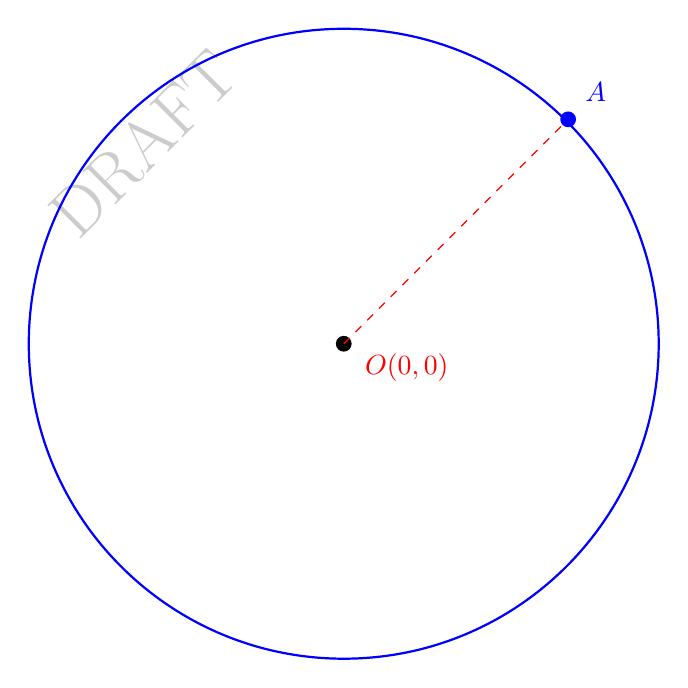
\begin{tikzpicture}[transform shape,scale=1]
	\fill[black] (0,0) circle (1 mm);
	\node at (0.8,-0.3) {$\textcolor{red}{O(0,0)}$};	
	\draw[thick,blue] (0,0) circle (4);
		\draw[dashed,red] (0,0)--(2.8,2.8);
\node at (3.2,3.2) {$\textcolor{blue}{A}$};	
	\fill[blue] (2.85,2.85) circle (1 mm);
\end{tikzpicture}\\
	\\
	কেন্দ্র মূলবিন্দুতে $O(0,0)$ এবং ব্যাসার্ধ $r$ বিশিষ্ট বৃত্ত। কেন্দ্র থেকে পরিধির উপর অবস্থিত $A(x,y)$ বিন্দুর দূরত্ব হলো ব্যাসার্ধ। \\ 
	\\ 
	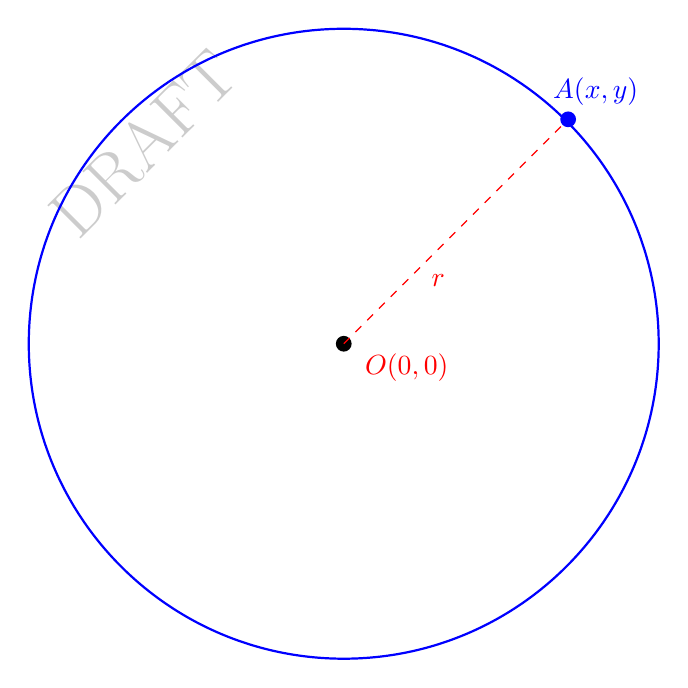
\begin{tikzpicture}[transform shape,scale=1]
		\fill[black] (0,0) circle (1 mm);
		\node at (0.8,-0.3) {$\textcolor{red}{O(0,0)}$};	
		\draw[thick,blue] (0,0) circle (4);
		\draw[dashed,red] (0,0)--(2.8,2.8);
		\node at (3.2,3.2) {$\textcolor{blue}{A(x,y)}$};	
		\fill[blue] (2.85,2.85) circle (1 mm);
	\node at (1.2,0.8) {$\textcolor{red}{r}$};		
	\end{tikzpicture}\\
	\\
	\begin{align*}
		OA&=r\\
		\sqrt{(x-0)^2+(y-0)^2}&=r\\
			\sqrt{x^2+y^2}&=r\\
			x^2+y^2&=r^2
	\end{align*}
\\
 কেন্দ্র মূল বিন্দু বিশিষ্ট বৃত্তের সমীকরণ \\
 $\textcolor{blue}{x^2+y^2=r^2}$\\
 (1)  নিচের চিত্রে কেন্দ্র মূল বিন্দু বিশিষ্ট  বৃত্তের সমীকরণ লিখ \\ 
	\begin{tikzpicture}[transform shape,scale=1]
		\draw [-latex,thick,red](-6,0) -- (6,0) node[right] {$x$} coordinate(x axis);
		\draw [-latex,thick,red](0,-6) -- (0,6) node[above] {$y$} coordinate(y axis);
		\fill[black] (0,0) circle (1 mm);
		\node at (0.8,-0.3) {$\textcolor{red}{O(0,0)}$};	
		\node at (4.7,-0.5) {$\textcolor{blue}{(4,0)}$};
		\fill[blue] (4,0) circle (1.5 mm);
		\draw[thick,blue] (0,0) circle (4);
	\end{tikzpicture}\\
	(2)  নিচের চিত্রে কেন্দ্র মূল বিন্দু বিশিষ্ট বৃত্ত  থেকে $D(a,b)$ বিন্দুর স্থানাঙ্ক নির্ণয় কর।  \\ 
	  \begin{tikzpicture}[transform shape,scale=1]
	  	\draw [-latex,thick,red](-6,0) -- (6,0) node[right] {$x$} coordinate(x axis);
	  	\draw [-latex,thick,red](0,-6) -- (0,6) node[above] {$y$} coordinate(y axis);
	  	\fill[black] (0,0) circle (1 mm);
	  	\node at (0.8,-0.3) {$\textcolor{red}{O(0,0)}$};	
	  	\node at (0.7,4.3) {$\textcolor{blue}{(0,5)}$};	
	  	\fill[blue] (0,4) circle (1.5 mm);
	  	\node at (-4.8,-0.5) {$\textcolor{blue}{D(a,b)}$};
	  	\fill[blue] (-4,0) circle (1.5 mm);
	  	\draw[thick,blue] (0,0) circle (4);
	  \end{tikzpicture}\\
  \\
	   (3)  নিচের চিত্রে কেন্দ্র মূল বিন্দু বিশিষ্ট বৃত্ত থেকে $AB$ রেখার দৈর্ঘ্য নির্ণয়  কর।  \\ 
	\begin{tikzpicture}[transform shape,scale=1]
		\draw [-latex,thick,red](-6,0) -- (6,0) node[right] {$x$} coordinate(x axis);
		\draw [-latex,thick,red](0,-6) -- (0,6) node[above] {$y$} coordinate(y axis);
		\fill[black] (0,0) circle (1 mm);
		\node at (0.8,-0.3) {$\textcolor{red}{O(0,0)}$};	
			\node at (4.7,-0.5) {$\textcolor{blue}{A}$};
				\fill[blue] (4,0) circle (1.5 mm);
				\node at (-4.8,-0.5) {$\textcolor{blue}{(-6,0)}$};
					\fill[blue] (-4,0) circle (1.5 mm);
			\node at (0.8,-4.3) {$\textcolor{blue}{B}$};	
				\fill[blue] (0,-4) circle (1.5 mm);		
		\draw[thick,blue] (0,0) circle (4);
		\draw[thin,purple] (4,0)--(0,-4);
	\end{tikzpicture}\\
\end{document}